\subsection{Architecture of the continuos query engine}


XXXXXX Gr\'afico de Javier
XXXXXx

\fmc{Explicar la idea de nuestro sistema, lo de que es un sistema para la detección de fraude a tiempo real, idea del double check para la authentication... sin entrar en mucho detalle de como lo hacemos (ya se describe en el apartado siguiente del continuous query engine). Que describa la idea / propósito / objetivo de lo que queremos hacer. Que sirva para introducir el apartado siguiente del \DPATM}

\fmc{IMPORTANTE: Buen dibujo de la arquitectura que sirva como para describir la idea del sistema que hacemos}
%
\iffalse
\begin{figure}[t!]
         \centering
         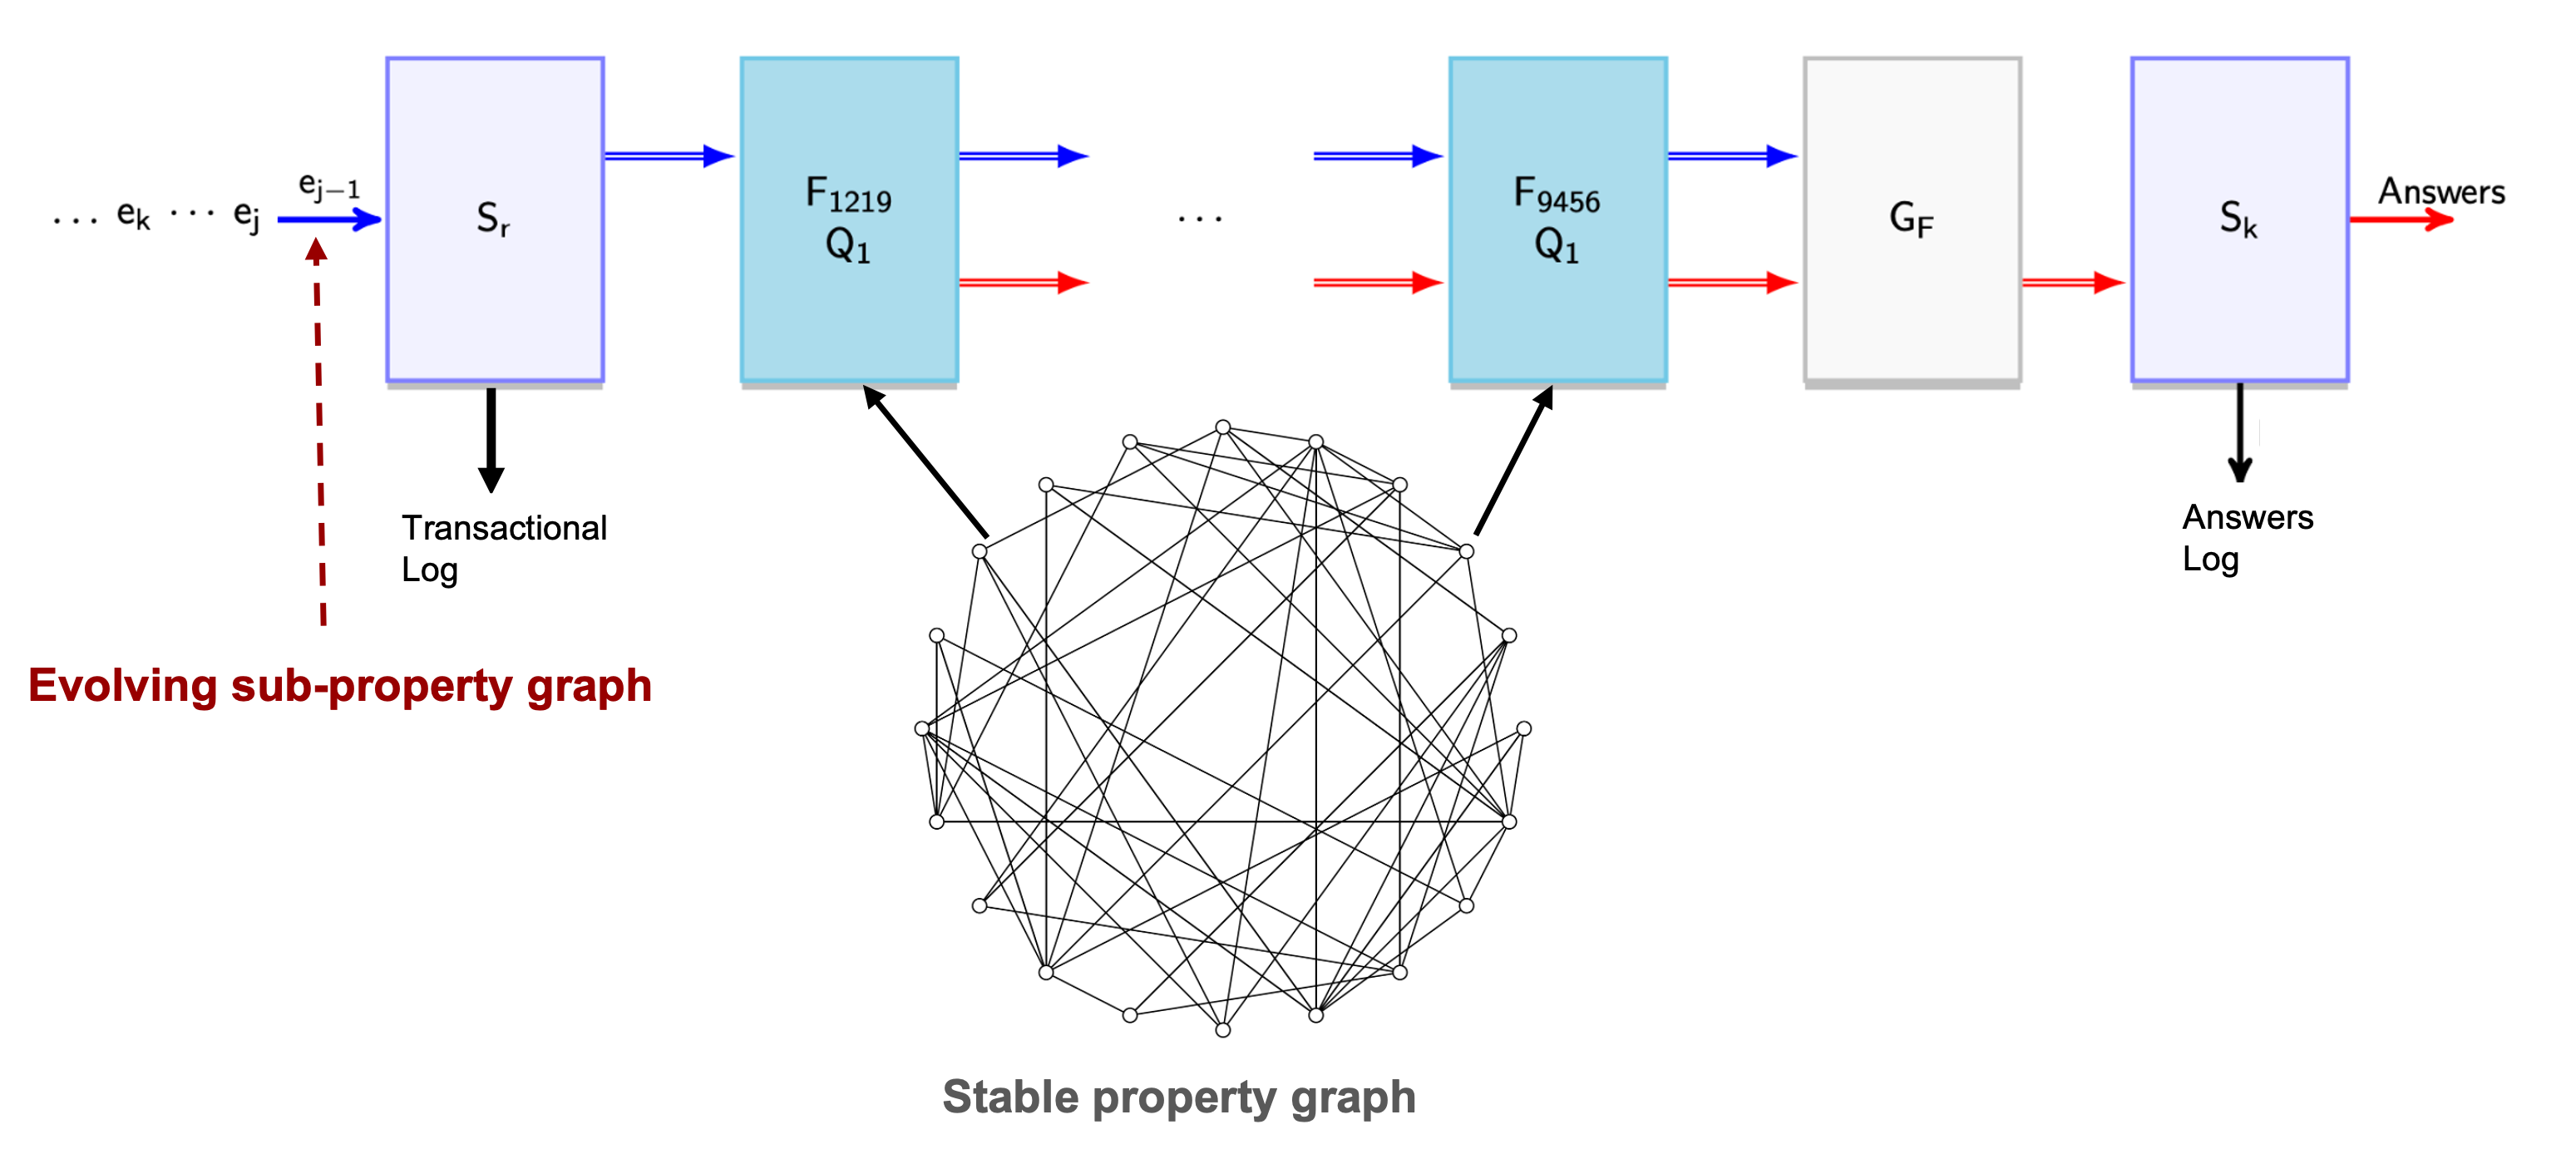
\includegraphics[width=0.7\textwidth]{images/architecture.png}
         \caption{Preliminary continuous query engine architecture for detecting anomalous ATM transactions based on the dynamic pipeline computational model. Considering the schema given in Figure \ref{fig:constinuousPGa}, in this directed (multi) graph presentation of the $\mathsf{DP_{ATM}}$, the arriving input data is a stream  $\mathsf{\langle \dots e_k\dots e_j \: e_{j-1}\rangle}$ corresponding to \textsf{interactions} (volatile relations). Boxes (vertices) represent stateful processes called \emph{stages} and internal arrows in the pipeline represent channels. Blue channels carry interaction edges and red channels carry detected anomalies (answers).  $\mathsf{S_r}$ and $\mathsf{S_k}$ correspond to the \textsf{Source} and \textsf{Sink} stages which receive input data and results, respectively. \textsf{Filter} stages, $\mathsf{F_{N}}$, are parameterized with the value of the property \textsf{number} ($\mathsf{N}$) of \textsf{Card} vertices. The \textsf{Generator} stage, $\mathsf{G_F}$, is in charge of spawning new filters, when required. The stable PG is a standard bank database (i.e. without volatile relations). Transactional log and Answers log keep input interactions and answers, respectively.
         }
         \label{fig:DP_ATM}
\end{figure}
\fi
%
